%---------------------------------------------------------
%	PRESENTATION BODY SLIDES
%---------------------------------------------------------
\section{Электронное охлаждение} % Note all sections and subsections are automatically placed in your table of contents

%------------------------------------------------
\begin{frame}
    \frametitle{Электронное охлаждение пучка в накопительном кольце}
	
	\par Метод электронного охлаждения, широко применяемый во всем мире для фокусировки ионных пучков в ускорителях элементарных частиц, был предложен нашим выдающимся физиком Г.И. Будкером в 1966 г. Однако создать действующую установку и получить первый результат удалось лишь спустя восемь лет благодаря  ученым ИЯФ СО РАН.
	\newline
	\par Суть заключалась в том, что пучок протонов и пучок электронов, двигаясь рядом с почти одинаковыми скоростями, начинают эффективно взаимодействовать посредством электромагнитных сил. Такое взаимодействие приводит к выравниванию их температур, т.е. перетеканию энергии теплового движения от протонного пучка к более холодному электронному. При этом, поскольку масса протона почти в две тысячи раз больше массы электрона, скорость его тепло­вого движения и, соответственно, угловой разброс пучка в десятки раз меньше, чем у пучка электронов: скорость частицы, имеющей в 2000 раз большую массу, должна быть в 40 раз меньше (в сопутствующей системе) в тот момент, когда в процессе охлаждения температура частиц станет равной температуре электронов.
		
\end{frame}
	
\begin{frame}
	\frametitle{Электронное охлаждение. Применение}
	
	\begin{figure}
		\centering
		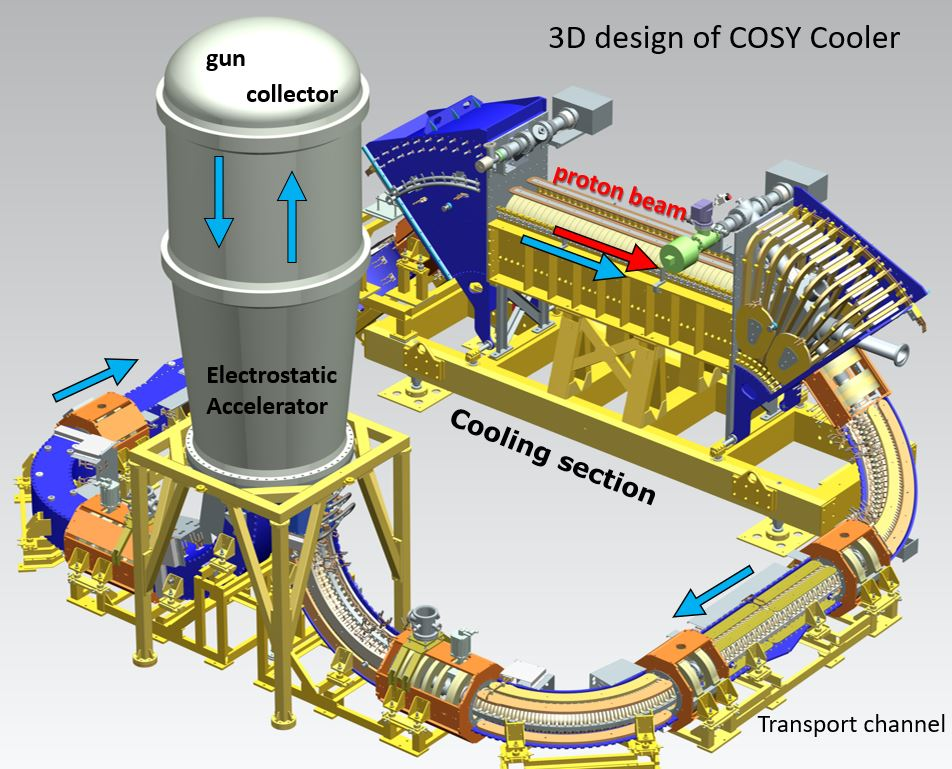
\includegraphics[width=0.49\linewidth]{images/COSY_el_cool}
		\includegraphics[width=0.39\linewidth]{"images/ELENA EC"}
		\caption{a) COSY; б) ELENA}
	\end{figure}

\end{frame}

\begin{frame}
	\frametitle{Электронное охлаждение В NICA}
	
	\begin{figure}
		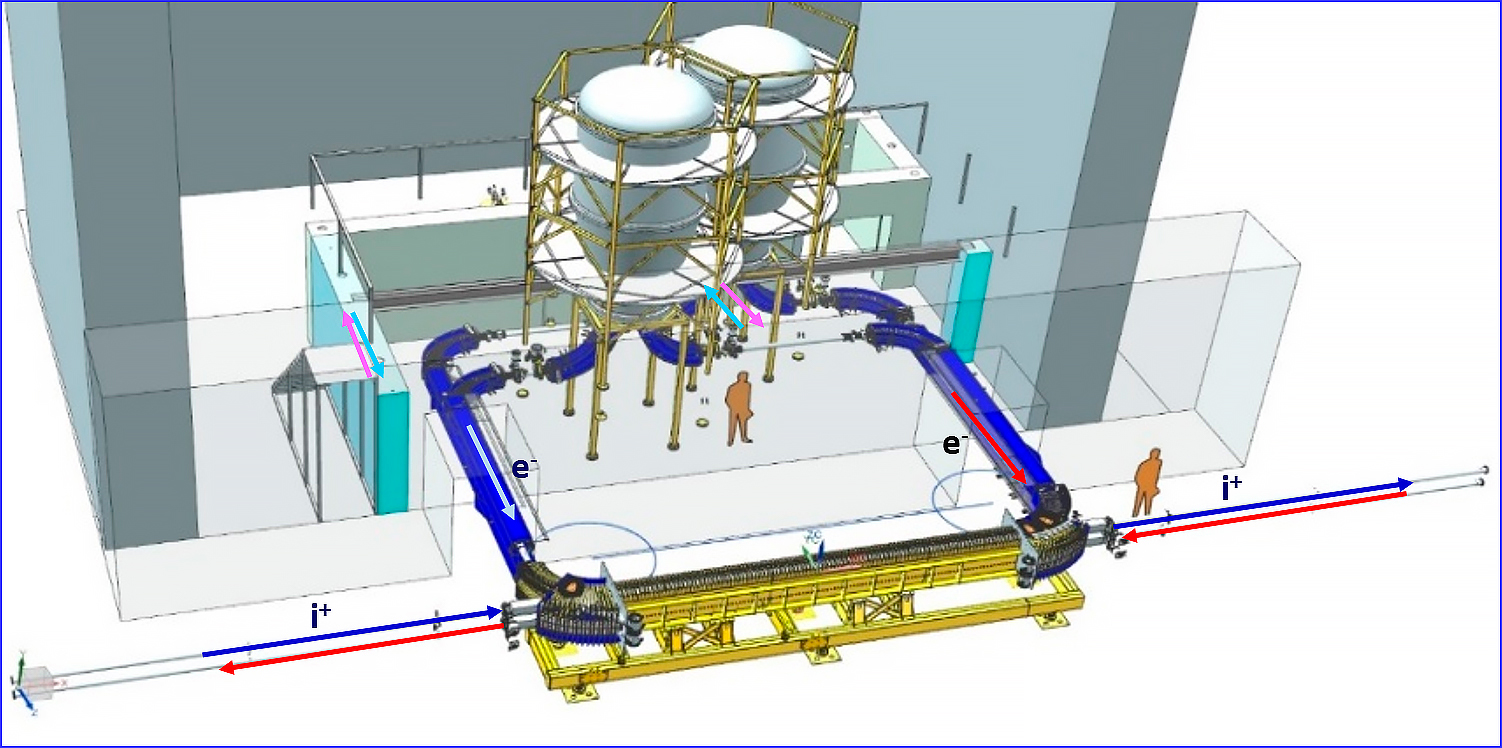
\includegraphics[width=0.59\linewidth]{images/NICA_el_cool}
		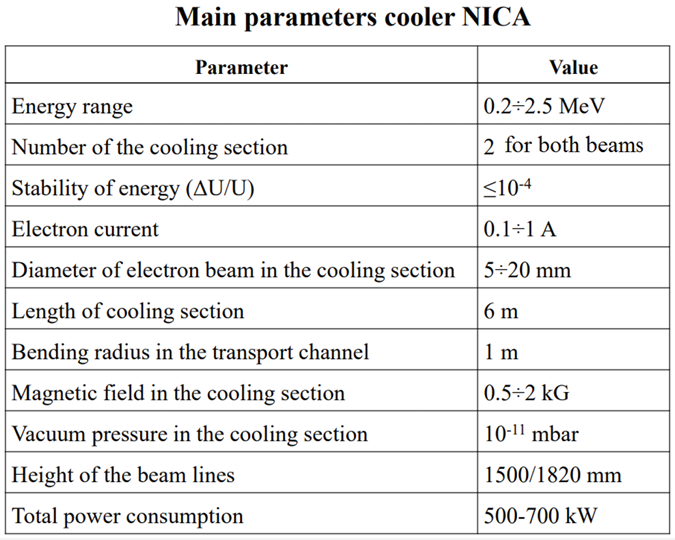
\includegraphics[width=0.39\linewidth]{images/NICA_el_main_param}
	\end{figure}
\end{frame}

\begin{frame}
	\begin{figure}
		\centering
		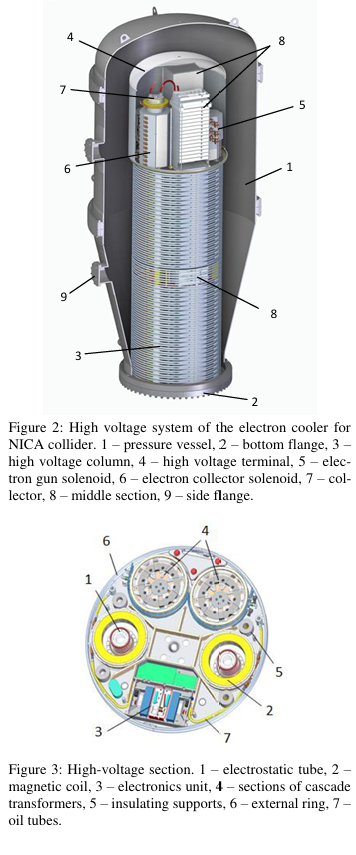
\includegraphics[width=0.2\linewidth]{images/HV}
	\end{figure}
	
\end{frame}

	